%% Springer Nature article template (sn-jnl), clean skeleton
%% Sections follow the Bioinformatics (OUP) Original Paper structure
%% Reference style options: sn-nature, sn-basic, sn-mathphys-num, sn-mathphys-ay,
%% sn-aps, sn-vancouver-num, sn-vancouver-ay, sn-apacite, sn-chicago
%% (see user-manual.pdf)

% sn-jnl loads geometry internally, so pass options before \documentclass
\PassOptionsToPackage{margin=1in}{geometry}

\documentclass[pdflatex,sn-nature]{sn-jnl}

\geometry{bindingoffset=0pt}

%%%% Packages
\usepackage{graphicx}
\usepackage{multirow}
\usepackage{amsmath,amssymb,amsfonts}
\usepackage{amsthm}
\usepackage{mathrsfs}
\usepackage[title]{appendix}
\usepackage[table]{xcolor}
\usepackage{textcomp}
\usepackage{manyfoot}
\usepackage{booktabs}
\usepackage{algorithm}
\usepackage{algorithmicx}
\usepackage{algpseudocode}
\usepackage{listings}

%%%% Theorem styles
\theoremstyle{thmstyleone}
\newtheorem{theorem}{Theorem}
\newtheorem{proposition}[theorem]{Proposition}
\theoremstyle{thmstyletwo}
\newtheorem{example}{Example}
\newtheorem{remark}{Remark}
\theoremstyle{thmstylethree}
\newtheorem{definition}{Definition}

\raggedbottom

\setlength\floatsep{10pt plus 2pt minus 2pt}
\setlength\textfloatsep{10pt plus 2pt minus 2pt}
\setlength\intextsep{10pt plus 2pt minus 2pt}

\newcommand{\TODO}[1]{\textcolor{red}{[TODO: #1]}}

\begin{document}

\title[DistributedPanGA]{DistributedPanGA: distributed pangenome self-alignment that reproduces FastGA}

%% \author* and \affil* mark the corresponding author and affiliation.
\author[1]{\fnm{Saksham} \sur{Diwan}}\email{sd966@cornell.edu}

\author[1]{\fnm{Harshaan} \sur{Chugh}}\email{hsc53@cornell.edu}

\author[2]{\fnm{Shuo} \sur{Cao}}

\author*[2]{\fnm{Erik} \sur{Garrison}}\email{egarris5@uthsc.edu}

\author*[1,3]{\fnm{Giulia} \sur{Guidi}}\email{gg434@cornell.edu}

\affil*[1]{\orgdiv{Department of Computer Science}, \orgname{Cornell University}, \orgaddress{\street{107 Hoy Rd}, \city{Ithaca}, \postcode{14853}, \state{New York}, \country{USA}}}

\affil*[2]{\orgdiv{Department of Genetics, Genomics and Informatics}, \orgname{University of Tennessee Health Science Center}, \orgaddress{\city{Memphis}, \postcode{38163}, \state{Tennessee}, \country{USA}}}

\affil[3]{\orgdiv{Applied Mathematics and Computational Research Division}, \orgname{Lawrence Berkeley National Laboratory}, \orgaddress{\street{1 Cyclotron Road}, \city{Berkeley}, \postcode{94720}, \state{California}, \country{USA}}}

%% Bioinformatics structured abstract (150 words recommended in total)
% \abstract{\textbf{Motivation:} Self-aligning a pangenome of $H$ haplotypes with FastGA finds matches across all haplotype pairs in a single scan of one sorted $k$-mer table, so the scan grows as $O(H \cdot L)$ rather than the $O(H^2 \cdot L)$ of explicit all-pairs alignment~\cite{fastga,garrison}. The table itself, however, grows with $H \cdot L$ and soon exceeds the memory of a single node. Distributing it across nodes removes that limit, but the result is only useful if it reproduces FastGA's alignments exactly.
%
% \textbf{Results:} DistributedPanGA partitions FastGA's index, seed generation and alignment across MPI ranks while keeping FastGA's alignment code. On yeast and primate pangenomes of 83\,Mbp to 2.63\,Gbp, every run is byte-identical to FastGA and, at equal core counts, 1.0--1.9$\times$ faster. On 90 human haplotypes of chromosome~6 (15.5\,Gbp), four nodes finish in 180\,s against FastGA's fastest measured one-node time of 1,480\,s; output is identical at 32 ranks, while at 64 ranks one of 1.38 million alignments is missing and is under investigation. Alignment dominates the run time, and its uneven cost across ranks limits further scaling.
%
% \textbf{Availability and Implementation:} DistributedPanGA is implemented in C with MPI and is available at \url{https://github.com/SakshamDiwan/DistributedPanGA}. Benchmark pangenomes are from Zenodo~\cite{pggbdata}. \TODO{license and archived release}
%
% \textbf{Contact:} egarris5@uthsc.edu, gg434@cornell.edu
%
% \textbf{Supplementary Information:} Supplementary data are available at \textit{Bioinformatics} online.}

\abstract{Aligning all haplotypes of a pangenome against each other with
FastGA takes one scan of a single sorted $k$-mer table~\cite{fastga,garrison},
but the table grows with the total sequence length and soon exceeds the
memory of one node. DistributedPanGA spreads FastGA's index, seed generation
and alignment across MPI ranks, keeps FastGA's alignment code, and must
reproduce FastGA's output exactly. On yeast and primate pangenomes, every run
is byte-identical to FastGA and, at equal core counts, up to 1.9$\times$
faster. On 90 human chromosome-6 haplotypes, four nodes take 180\,s against
1,480\,s for FastGA's fastest measured one-node run; the output is identical
at 32 ranks, and at 64 ranks one of 1.38 million alignments is missing and
under investigation. Alignment dominates the run time, and its uneven cost
across ranks limits further scaling.}

\maketitle

%% Original Paper: up to 7 pages (approx. 5,000 words, excluding figures).
%% Section order: Introduction, System and methods, Algorithm,
%% Implementation, Discussion, References.

%% Introduction -- owner: Saksham.
%% Only claims supported by the project (abstract, Section 2/3 methods,
%% last semester's report, our measurements).

\section{Introduction}\label{sec:introduction}

Aligning all haplotypes of a pangenome against each other can be done in
one pass: FastGA~\cite{fastga} puts every haplotype's sampled $k$-mers into
one sorted table, where matching $k$-mers sit next to each other, so a
single scan finds matches between every pair of
haplotypes~\cite{garrison}. The table grows with the total sequence length
and soon outgrows the memory of one machine.

We distribute this table, and the steps that use it, across nodes so it can
grow past one machine. The result is only useful if it is exactly FastGA's,
so we require byte-identical output.

This paper presents DistributedPanGA, an MPI version of FastGA's
self-alignment, and evaluates it on three pangenomes. Its output matches
FastGA's in every configuration tested, and with the same number of cores
it runs up to 1.9$\times$ faster.


\section{Prior work}\label{sec:prior}

\paragraph{FastGA.} FastGA~\cite{fastga} aligns genomes on one machine. It
builds a sorted $k$-mer index, generates seeds from it, chains the seeds
and aligns them (Section~\ref{sec:methods:fastga}). DistributedPanGA reuses
its seed-merge and alignment code unchanged.

\paragraph{Pangenome self-alignment.} Garrison~\cite{garrison} showed that
running FastGA once on all haplotypes together is about 17$\times$ faster
than aligning every pair separately on yeast, because one scan of one
sorted table finds matches between all pairs (Section~\ref{sec:methods:fastga}).
We therefore keep FastGA's single sorted table,
spread across nodes, rather than run each pair of haplotypes separately.


\section{System and methods}\label{sec:methods}

%% For machine learning papers, add a subsection describing the training
%% dataset, the cross-validation sets, and the independent test set.

\section{Algorithm}\label{sec:algorithm}

%% =====================================================================
%% Algorithm / Seed extraction -- owner: Harshaan.
%% =====================================================================

\subsection{Seed extraction}\label{sec:alg:extraction}

Extraction reproduces FastGA's seed selection exactly. Each rank streams its
contigs in windows of up to 10\,Mbp and slides over every 12-mer, comparing
the canonical 8-mers it contains. A position is selected when the smallest
8-mer lies at either end of the 12-mer (a closed syncmer); ties are kept, as
in FastGA.
% CHECK: syncmer terminology against the FastGA paper.

Each selected position yields two records: the forward 40-mer starting at
the position and the reverse-complement 40-mer that ends 12 bases after it.
A record stores the 2-bit packed k-mer together with its contig, position
and strand. Per-occurrence records are required because seeds are pairs of
positions; k-mer counts alone cannot produce alignments.

The 40 bases of a k-mer may cross the boundary between two scan windows.
Every window after the first therefore also holds the 40 bases that precede
it, which covers all reverse-complement k-mers and all forward k-mers that
start before the window. Only a forward k-mer that runs past the right edge
of a non-final window is read separately from the GDB. The selection loop,
the selected positions and the order in which records are emitted are
identical for every window size.

%% =====================================================================
%% Algorithm / Data movement -- owner: Harshaan (design level only).
%% Saksham owns the O2/O4 implementation text; keep code-level detail there.
%% Describes the CURRENT pipeline: in-memory seeds (bce56a4, a2cf364).
%% Verified against src/dsort.c, src/chunked_exchange.[ch],
%% src/contig_assignment.c, src/pga-mpi-merge.c, src/fastga_pipeline.c.
%% =====================================================================

\subsection{Data movement between ranks}\label{sec:alg:mpi}

Ranks exchange data twice: records during the distributed sort, and seeds
before alignment.

\paragraph{Distributed sort.} Each record is assigned to one of 1{,}024
buckets by the first five bases of its k-mer. One all-reduce of bucket
counts lets every rank compute the same split into $P$ contiguous bucket
ranges of about $1/P$ of the records, by the rule FastGA uses to divide its
index among threads. Each rank then radix-sorts its slice and recomputes
LCPs, correcting the first against the preceding rank's last k-mer.
Because buckets are never split, seed generation needs no communication:
FastGA's merge pairs only occurrences sharing their first 12 bases, so
every candidate group, including the full count tested against the cutoff,
lies on one rank, and each rank produces exactly its share of FastGA's
seeds.

\paragraph{Seed redistribution.} Each seed is sent to the rank that owns
its contig pair. Every rank computes the same pair-to-rank map from contig
lengths alone, giving pairs in decreasing order of length product to the
rank with the smallest accumulated product, so no communication is needed.
The merge writes each seed directly into an in-memory buffer for its
destination rank.

\paragraph{Bounded exchanges.} Both exchanges are personalized all-to-all
transfers of fixed-size records whose volume per rank can exceed the 32-bit
counts of \texttt{MPI\_Alltoallv}. Large transfers are split into rounds
of whole records, and the result is byte-identical to a single unbounded
exchange for any number of rounds (Section~\ref{sec:impl:o2}). The per-round
budget bounds only
staging memory: the complete send and receive data stay resident (during
the sort, a rank holds its extracted records, their packed send copy and
its received slice), so peak memory per rank is set by its volume of
records and seeds, not by the budget (Section~\ref{sec:implementation}).
% CHECK with Saksham: memory sentences vs. his O4 subsection (avoid overlap).


%% Algorithm / distributed alignment -- owner: Saksham.

\subsection{Distributed alignment}\label{sec:alg:alignment}
Each rank aligns the contig pairs it owns (Section~\ref{sec:alg:mpi}) with
FastGA's code. The map covers all $N(N+1)/2$ pairs of the $N$ contigs,
including each contig with itself; ties are broken by contig index, so
every rank computes the same map. Both orientations of a pair map to the
same rank. Seeds are split into two sets: same strand and opposite strands.

Each rank groups its seeds by contig pair, sorts them by diagonal, and
aligns each pair and strand set with FastGA's routine, which chains seeds,
extends chains into local alignments and removes redundant ones. Each rank
writes its own \texttt{.1aln} file and converts it to PAF with
\texttt{ALNtoPAF}; the output is the union of these files.

A pair's alignments depend only on its seeds and its two contigs, and all
its seeds reach one rank, so each rank produces exactly FastGA's alignments
for its pairs. The map balances contig length products, not alignment cost.


\section{Implementation}\label{sec:implementation}

%% Figures: 86 mm (single column) or 178 mm (double column) wide, white
%% background, with alt text placed directly under the caption, e.g.
%% \begin{figure}[t]
%%   \centering
%%   \includegraphics[width=86mm]{fig/example.pdf}
%%   \caption{Caption text.}\label{fig:example}
%%   \par\noindent Alt text: Short description of the figure.
%% \end{figure}

%% =====================================================================
%% Implementation / Extraction I/O (O1) -- owner: Harshaan.
%% No numbers here: measured results belong in the evaluation.
%% =====================================================================

\subsection{Extraction I/O}\label{sec:impl:o1}

Per-rank timers showed that extraction dominated early runs and scaled
poorly with the number of ranks. System-call tracing located the cause in the
packing step. The scan already held the current window in memory, but the
40 bases of each selected k-mer were read again from the GDB, which costs
one file seek per record.

We now pack each k-mer directly from the window buffer, reading from the
GDB only in the boundary case of Section~\ref{sec:alg:extraction}; the
window refill was extended by 40 bases of left context. Both paths use the same
packing routine, and the selection loop is unchanged, so the change affects
only where bases are read from.

We validated the change at three levels. The extraction output is
byte-identical to the previous implementation and to a reference dump from
an instrumented copy of FastGA's index builder. Unit tests run with a 64-base
window to force many boundary cases, check that both packing paths are
exercised and together account for every record, and also run under address
and undefined-behaviour sanitizers. Finally, end-to-end runs match the
FastGA reference alignments.
% TODO(Harshaan): extraction speedups go in the evaluation, not here
%   (historical numbers: author-notes/harshaan-evidence.txt E2).


\subsection{Large-count exchanges}\label{sec:impl:o2}
\TODO{Saksham: O2 implementation}

\subsection{In-memory seeds}\label{sec:impl:o4}
\TODO{Saksham: O4 implementation}

\section{Results}\label{sec:results}

%% Results / Experimental setup -- owner: Saksham. The human runs (Harshaan)
%% use the same settings (jobs/report/config.sh).

\subsection{Experimental setup}\label{sec:results:setup}

We ran DistributedPanGA and FastGA on the three pangenomes in
Table~\ref{tab:datasets} and compared their output and their running time.
DistributedPanGA ran on one to four nodes; FastGA, which uses threads on a
single machine, ran on one node. All runs used dedicated CPU nodes on Perlmutter,
each with 128 cores and 512\,GB of memory. Both tools used FastGA's default parameters.

A run with $P$ ranks on $n$ nodes places
$P/n$ ranks on each node and pins each rank to an equal share of the node's
cores. A rank is single-threaded except during the local $k$-mer sort, which
uses four threads.

We report the time of each of four stages and their sum, the total time.
The stages are extraction; the distributed sort; seed generation and
redistribution (Section~\ref{sec:methods:overview}, stages 3--4); and
alignment with PAF output (stages 5--6). Ranks that finish extraction
early wait at the start of the sort for the slowest one; we count that wait
as extraction, not as sort. Each configuration ran three times. We report
the run with the median total time, so its stage times add up to its total.

FastGA ran on one node with $t$ threads. Its time is the sum of
\texttt{GIXmake}, \texttt{FastGA} and \texttt{ALNtoPAF}. \texttt{GIXmake}
accepts at most 32 threads, so for $t>32$ it ran with 32. \texttt{FastGA}
crashes at startup with 125 or more threads on all three datasets, so we
measured it up to $t=64$. \texttt{FAtoGDB} is excluded because both tools
start from the same GDB.

A run is correct if the concatenation of its per-rank PAF files, sorted, is
byte-identical to FastGA's sorted PAF for the same input.

\begin{table}[h]
\caption{Datasets. yeast7 is seven \textit{S.~cerevisiae} strains; the
primate sets are chromosome~6 assemblies from the PGGB benchmark
collection~\cite{pggbdata}. Contigs are the GDB's gap-free sequences.}\label{tab:datasets}
\begin{tabular}{@{}lrrrr@{}}
\toprule
Dataset & Bases & Sequences & Contigs & FastGA alignments \\
\midrule
yeast7 & 83.4\,Mbp & 112 & 119 & 43,126 \\
primates4.chr6 & 672.5\,Mbp & 4 & 100 & 1,547,485 \\
primates14.chr6 & 2.63\,Gbp & 52 & 82 & 4,577,556 \\
\botrule
\end{tabular}
\end{table}


\subsection{Yeast and primate datasets}\label{sec:results:small}

All 30 DistributedPanGA runs produced output byte-identical to FastGA's.
Table~\ref{tab:pipeline} gives the time of each stage and the total for
every configuration.

\begin{table}[htbp]
\caption{DistributedPanGA time per stage, in seconds. ``Seeds'' is seed
generation and redistribution; ``Alignment'' includes PAF output.
``Total'' is the sum of the four stages. Each row is the run with the
median total time of three.}\label{tab:pipeline}
\begin{tabular}{@{}lrrrrrrr@{}}
\toprule
Dataset & Nodes & Ranks & Extraction & Sort & Seeds & Alignment & Total \\
\midrule
\csname @@input\endcsname fig/table_pipeline.tex
\botrule
\end{tabular}
\end{table}

\begin{figure}[htbp]
\centering
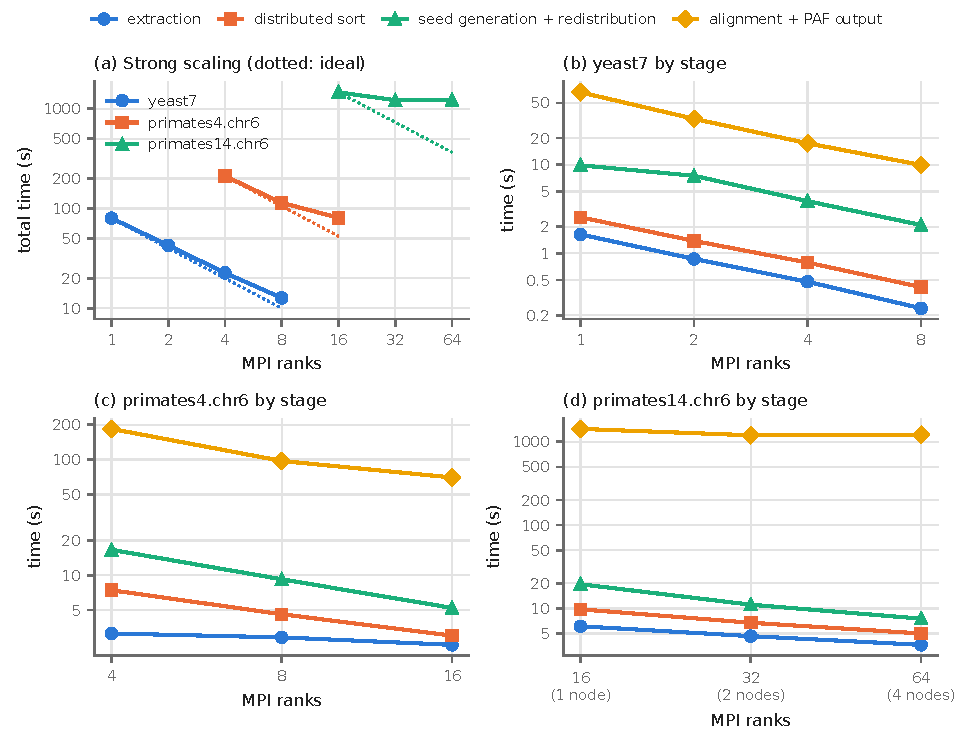
\includegraphics[width=\textwidth]{fig/strong_scaling.pdf}
\caption{All panels use log--log axes. (a) Total time against ranks. yeast7 and primates4.chr6 run on one
node. primates14.chr6 uses 16 ranks per node (1, 2 and 4 nodes). Dotted lines
show ideal scaling from the smallest run. (b)--(d) Time per stage for each
dataset; the legend at the top applies to these panels.}\label{fig:strong}
\end{figure}

\paragraph{Strong scaling on one node.} From 1 to 8 ranks, yeast7 drops
from 79.97\,s to 12.69\,s, a speedup of 6.3 (79\% parallel efficiency;
Fig.~\ref{fig:strong}a). From 4 to 16 ranks, primates4.chr6 drops from
211.47\,s to 80.76\,s, a speedup of 2.6 (65\%). Alignment takes 77--87\% of
the total time in these runs.

\paragraph{Strong scaling across nodes.} With 16 ranks per node,
primates14.chr6 takes 1,463.94\,s on one node, 1,218.54\,s on two and
1,229.09\,s on four. Alignment takes 98--99\% of the total time and stays between
1,196.09\,s and 1,428.58\,s (Fig.~\ref{fig:strong}d). From 16 to 64 ranks,
extraction falls from 6.10\,s to 3.65\,s, the sort from 9.76\,s to 5.00\,s,
and seed generation and redistribution from 19.50\,s to 7.53\,s.

Table~\ref{tab:perrank} breaks the alignment stage down by rank. From 16 to
64 ranks on primates14.chr6, the average rank's alignment time falls from
722.15\,s to 183.43\,s, while the slowest rank's stays between 1,169.50\,s
and 1,393.88\,s. At 64 ranks the slowest rank takes 6.59 times the
average; on primates4.chr6 the ratio grows from 1.09 at 4 ranks to 1.70 at
16.

\begin{table}[htbp]
\caption{Alignment time per rank, in seconds, for the runs in
Table~\ref{tab:pipeline}: the slowest, average and fastest rank, and the
slowest divided by the average. Alignment time here is the time spent
aligning seed chains, without sorting seeds or writing PAF.}\label{tab:perrank}
\begin{tabular}{@{}lrrrrrr@{}}
\toprule
Dataset & Nodes & Ranks & Slowest & Average & Fastest & Slowest/avg. \\
\midrule
\csname @@input\endcsname fig/table_perrank.tex
\botrule
\end{tabular}
\end{table}

\begin{figure}[htbp]
\centering
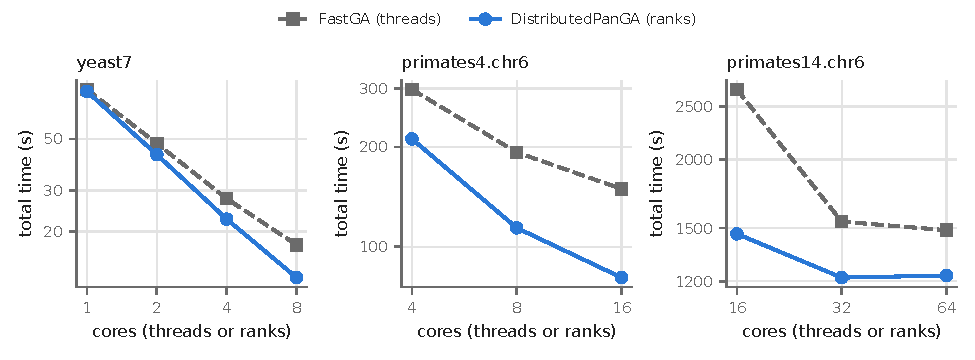
\includegraphics[width=\textwidth]{fig/vs_fastga.pdf}
\caption{DistributedPanGA ($P$ ranks) against FastGA ($t$ threads on one
node) at equal core counts, on log--log axes. For primates14.chr6,
DistributedPanGA uses 16 ranks per node.}\label{fig:fastga}
\end{figure}

\begin{table}[htbp]
\caption{FastGA time per step on one node, in seconds. Each row is the run
with the median total time of three. \texttt{GIXmake} builds the index,
\texttt{FastGA} aligns and \texttt{ALNtoPAF} writes PAF.}\label{tab:fastga}
\begin{tabular}{@{}lrrrrr@{}}
\toprule
Dataset & Threads & \texttt{GIXmake} & \texttt{FastGA} & \texttt{ALNtoPAF} & Total \\
\midrule
\csname @@input\endcsname fig/table_fastga.tex
\botrule
\end{tabular}
\end{table}

\paragraph{Comparison with FastGA.} Table~\ref{tab:fastga} gives FastGA's time per step. All FastGA runs produced the same
alignments as the reference. At equal core counts, DistributedPanGA is
1.0--1.4$\times$ faster than FastGA on yeast7 (1 to 8 cores),
1.4--1.9$\times$ on primates4.chr6 (4 to 16 cores) and 1.2--1.8$\times$ on
primates14.chr6 (16 to 64 cores) (Fig.~\ref{fig:fastga}). From 4 to 16 cores
on primates4.chr6, FastGA speeds up by 2.0 and DistributedPanGA by 2.6. From
16 to 64 cores on primates14.chr6, FastGA speeds up by 1.8 and
DistributedPanGA by 1.2.

FastGA's fastest one-node time on primates14.chr6 is 1,486.52\,s, at 64
threads. DistributedPanGA takes 1,463.94\,s on one node, 1,218.54\,s on two
and 1,229.09\,s on four, 1.0, 1.2 and 1.2$\times$ faster than that time.

\paragraph{Weak scaling.} Two sets of three runs have about the same number
of bases per rank: 83\,Mbp (yeast7 on 1 rank, primates4.chr6 on 8,
primates14.chr6 on 32 over two nodes) and 42\,Mbp (2, 16 and 64 ranks).
At 83\,Mbp per rank, seed generation and redistribution take 9.87, 9.23 and
11.07\,s; extraction grows 2.9$\times$ (1.63 to 4.65\,s), the sort
2.6$\times$ (2.55 to 6.73\,s) and alignment 18$\times$ (65.92 to
1,196.09\,s).

Table~\ref{tab:weak} gives the alignment output per rank for these runs.
At 83\,Mbp per rank, from yeast7 to primates14.chr6 the aligned bases per
rank grow 7.9$\times$, the average rank's alignment time 8.6$\times$ and
the slowest rank's 28$\times$. primates4.chr6 aligns 1.07$\times$ as many
bases per rank as yeast7, in 4.5$\times$ as many alignments, and its
average rank takes 1.7$\times$ as long.

\begin{table}[htbp]
\caption{Weak scaling: alignment output and alignment time per rank. Aligned
bases are the summed lengths of all alignments in FastGA's output, which
every run reproduces, divided by the ranks; one input base is counted once
for every alignment it is part of. Alignment time is as in
Table~\ref{tab:perrank}.}\label{tab:weak}
\begin{tabular}{@{}lrrrrrr@{}}
\toprule
 & & Input & Aligned & Alignments & \multicolumn{2}{c}{Alignment time (s)} \\
\cmidrule{6-7}
Dataset & Ranks & Mbp/rank & Mbp/rank & per rank & Average & Slowest \\
\midrule
\csname @@input\endcsname fig/table_weak.tex
\botrule
\end{tabular}
\end{table}


%% =====================================================================
%% Results / Human chromosome 6 -- owner: Harshaan.
%% Sources: ~/pga-jobs/human/logs (jobs 61244453 index, 61244455 / 61255430
%% FastGA, 61255434 / 61244457 DistributedPanGA, repeats 61277457 /
%% 61277456), per-rank merge.err under $SCRATCH/pga-human. Stage times use
%% the same rule as Table tab:pipeline (wait for the slowest extractor is
%% extraction). Figure: fig/make_human_fig.py.
%% =====================================================================

\subsection{Human chromosome 6}\label{sec:results:human}

hsapiens90.chr6 holds 90 human haplotypes of chromosome~6 from the same
collection~\cite{pggbdata}: 15.51\,Gbp in 1,410 sequences and 1,422 contigs,
six times the size of primates14.chr6. FastGA's reference has 1,375,248
alignments and links every one of the 4,005 pairs of haplotypes. We ran
DistributedPanGA with 32 and 64 ranks on four nodes and FastGA on one node
with 16 and 32 threads; each configuration ran twice for DistributedPanGA
(totals within 1\%) and once for FastGA. \texttt{GIXmake} crashes with 32
threads on this input, so FastGA's index was built with 16 threads in both
FastGA rows.

\paragraph{Correctness.} With 32 ranks, both runs are byte-identical to
FastGA's sorted output. FastGA's output is the same at 16 and 32 threads.
With 64 ranks, both runs miss the same single alignment, a same-strand
self-alignment of one contig over about 3.9\,kbp; every other line matches.
The seeds for that contig pair are identical at 32 and 64 ranks, so the
difference arises during alignment. We have not yet determined whether it
comes from our pipeline or from an order-dependent edge case in FastGA's
alignment code.

\paragraph{Time and memory.} Table~\ref{tab:human} and
Fig.~\ref{fig:human} give the times. DistributedPanGA takes 291.17\,s with
32 ranks and 180.07\,s with 64, a speedup of 1.62. FastGA takes 1,480.42\,s
with 16 threads and 1,736.93\,s with 32, so DistributedPanGA with 64 ranks
is 8.2$\times$ faster than FastGA's fastest run, and 6.0$\times$ faster at
32 ranks against 32 threads. Alignment is 84--87\% of DistributedPanGA's
total. The slowest rank's alignment time is 1.32 times the average at 32
ranks and 1.49 at 64. FastGA peaks at 15.1\,GB on one node. DistributedPanGA
peaks at 22.9\,GB per rank with 32 ranks and 14.1\,GB with 64; summed over
ranks, that is 675\,GB and 747\,GB.

\begin{table}[h]
\caption{hsapiens90.chr6, time per stage in seconds. DistributedPanGA ran on
four nodes; stages as in Table~\ref{tab:pipeline}. For FastGA (one node),
``Index'' is \texttt{GIXmake} (16 threads in both rows), ``Align'' is
\texttt{FastGA} and ``PAF'' is \texttt{ALNtoPAF}. Peak memory is per rank for
DistributedPanGA and per process for FastGA.}\label{tab:human}
\begin{tabular}{@{}lrrrrrrr@{}}
\toprule
DistributedPanGA & Ranks & Extraction & Sort & Seeds & Alignment & Total & Peak GB \\
\midrule
 & 32 & 9.86 & 22.65 & 6.46 & 252.20 & 291.17 & 22.9 \\
 & 64 & 6.13 & 18.16 & 3.85 & 151.92 & 180.07 & 14.1 \\
\midrule
FastGA & Threads & Index & Align & PAF & & Total & Peak GB \\
\midrule
 & 16 & 400.39 & 1,069.81 & 10.22 & & 1,480.42 & 13.4 \\
 & 32 & 400.39 & 1,330.71 & 5.83 & & 1,736.93 & 15.1 \\
\botrule
\end{tabular}
\end{table}

\begin{figure}[h]
\centering
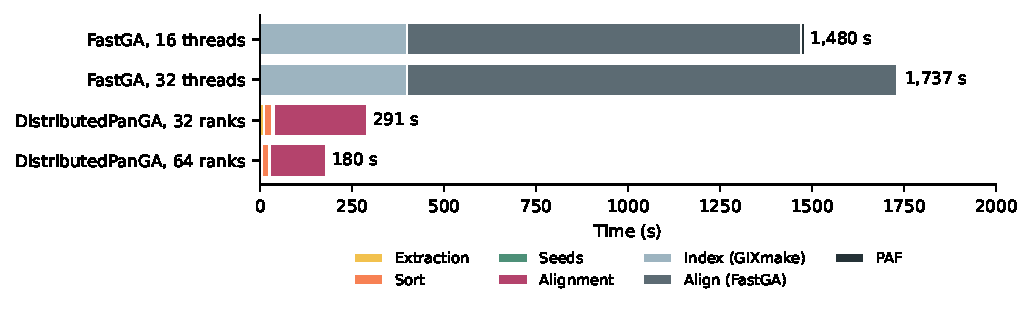
\includegraphics[width=\textwidth]{fig/human_chr6.pdf}
\caption{hsapiens90.chr6: time per stage for FastGA on one node and
DistributedPanGA on four nodes (Table~\ref{tab:human}).}\label{fig:human}
\par\noindent Alt text: Horizontal stacked bars. FastGA takes about 1,480
and 1,737 seconds, mostly alignment plus a 400-second index build;
DistributedPanGA takes about 291 and 180 seconds, mostly alignment.
\end{figure}


%% =====================================================================
%% Results / Scaling across datasets -- owner: Harshaan.
%% Measurements only; interpretation in sec/harshaan/disc-scaling.tex.
%% Sources: fig/table_pipeline.tex, fig/table_perrank.tex, Table tab:human;
%% human per-pair task times from PGA_PAIR_TASKS (jobs 61277457, 61277456);
%% primates14 largest task from docs/agent/decision-gate-2.md (earlier build,
%% same alignment code). Figure: fig/make_scaling_fig.py.
%% =====================================================================

\subsection{Scaling across datasets}\label{sec:results:scaling}

Fig.~\ref{fig:scaling} compares the four datasets. At the largest doubling
of ranks tested for each, the total time falls by 1.78$\times$ on yeast7
(4 to 8 ranks), 1.41$\times$ on primates4.chr6 (8 to 16), 0.99$\times$ on
primates14.chr6 (32 to 64) and 1.62$\times$ on hsapiens90.chr6 (32 to 64).
At its largest rank count, the slowest rank's alignment time is 1.70 times
the average on primates4.chr6, 6.59 on primates14.chr6 and 1.49 on
hsapiens90.chr6.

On hsapiens90.chr6, the per-pair records sum to 6,013\,s of alignment work
at 32 ranks and 6,426\,s at 64, and the most expensive contig pair, a
self-alignment, takes 34\,s, about 0.5\% of the total. On primates14.chr6
the most expensive pair takes 773\,s, about 7\% of all alignment work
(measured with an earlier build that runs the same alignment code). From 32
to 64 ranks on hsapiens90.chr6, the alignment stage falls from 252.20\,s to
151.92\,s, while the average rank's alignment time falls from 187.12\,s to
100.47\,s; the sort falls from 22.65\,s to 18.16\,s. Peak memory per rank
falls from 22.9\,GB to 14.1\,GB, and memory summed over ranks rises from
675\,GB to 747\,GB.

\begin{figure}[h]
\centering
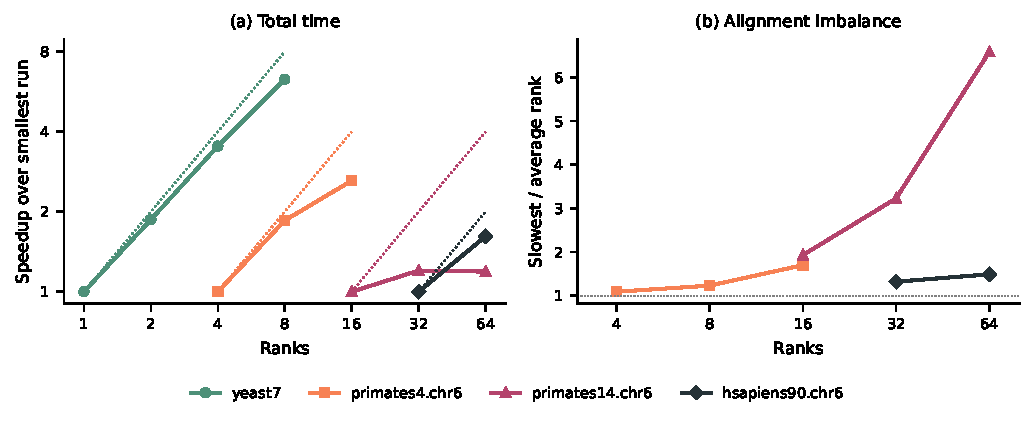
\includegraphics[width=\textwidth]{fig/scaling_summary.pdf}
\caption{Scaling across the four datasets. (a) Speedup of the total time
over each dataset's smallest run; dotted lines show ideal scaling.
(b) Slowest rank's alignment time divided by the average
(Table~\ref{tab:perrank} and Section~\ref{sec:results:human}).}\label{fig:scaling}
\par\noindent Alt text: Two line plots against ranks. Yeast7 and the human
dataset stay close to ideal speedup, primates4.chr6 falls below it, and
primates14.chr6 stops improving after 32 ranks. Alignment imbalance rises
to 6.6 on primates14.chr6 at 64 ranks but stays below 1.5 on the human
dataset.
\end{figure}


\section{Discussion}\label{sec:discussion}

%% Reserved (Saksham): interpretation of small-dataset results.
% TODO(Harshaan+Saksham): scaling bottlenecks, after human results (outline: sec/harshaan/disc-scaling.tex)
% \subsection{Scaling across datasets}\label{sec:disc:scaling}

The human dataset, six times larger than primates14.chr6, scales much
better, which fits the explanation in Section~\ref{sec:disc:small}: a
contig pair is never split, so the most expensive pair bounds the
alignment stage. hsapiens90.chr6 has 1,422 contigs against 82, and its most
expensive pair is about 0.5\% of the alignment work rather than 7\%. Its
work could in principle be spread over roughly 180 ranks before that pair
sets the stage time, against about 14 for primates14.chr6. How many contigs
an input has, and how evenly its work falls on them, may therefore matter
more for scaling than its size.

The task bound does not explain the remaining imbalance on the human data.
At 64 ranks its slowest rank aligns for 149\,s, more than four times its
most expensive pair (34\,s) and 1.49 times the average (100\,s). Since no
single task is that large, the gap most likely comes from the static
assignment by length product, which does not track alignment cost (Section~\ref{sec:disc:future}). A perfectly balanced
assignment would shorten the alignment stage by at most this factor of
about 1.5 at 64 ranks.

% TODO(Harshaan): human-scale validation, after the human jobs (branches: sec/harshaan/disc-human.tex)
% %% =====================================================================
%% Discussion / Human scale -- owner: Harshaan.
%% Numbers in sec/harshaan/results-human.tex. The 64-rank difference is
%% stated as open; do not attribute it to FastGA without proof
%% (trace so far: identical seeds, alignment-stage difference; see
%% docs/agent/state.md).
%% =====================================================================

\subsection{Human scale}\label{sec:disc:human}

FastGA handled hsapiens90.chr6 on a single node in under half an hour with
15\,GB of memory, so at the scale of one chromosome, distribution shortens
the run rather than making it possible. The input is six times larger than
primates14.chr6, yet FastGA's best time is about the same on both, and
DistributedPanGA is several times faster on it. A likely reason is that the
90 haplotypes are nearly identical: most $k$-mers should then occur at
least $f=10$ times and yield no seeds, leaving less alignment work. We did
not measure this directly. Where single-node FastGA reaches its
limits, in more haplotypes or whole genomes, remains to be measured.

DistributedPanGA's speed comes with memory: summed over ranks it used about
45--50 times FastGA's peak. Each rank holds its records and seeds in memory,
and ranks are single-threaded, so more ranks, not threads, are the way to use
a node's cores.

The single alignment missing at 64 ranks is the only disagreement with
FastGA across all datasets and rank counts. Because the seeds agree, it
arises in the alignment stage; whether it lies in our pipeline or in an
order-dependent edge case of FastGA's alignment code is under investigation.
Until it is explained, exact agreement is
established for human chromosome~6 at 32 ranks only.

%% =====================================================================
%% Discussion / Limitations and future work -- owner: Harshaan.
%% No HySortK here (Nov 13 decision). No O3/O5 labels: research-plan.md
%% and later docs disagree on what O3 means; O5 (GPU) is not discussed.
%% Nothing below is implemented.
%% =====================================================================

\subsection{Limitations and future work}\label{sec:disc:future}

Alignment is now the dominant stage, and its cost is unevenly distributed
across ranks. The time of an alignment task follows the amount of sequence
it aligns, which is not known in advance and is poorly predicted by seed
counts or contig lengths. This suggests replacing the static assignment of
contig pairs with dynamic scheduling, in which ranks take the next task from
a shared queue as they become free.
% CHECK: "dominant" + "poorly predicted" come from decision-gate-2
%        (primates); keep qualitative here, numbers in the evaluation.

Scheduling alone has a limit: each contig pair is aligned by one rank, and
self-alignments of long contigs are the largest tasks. Scaling further
requires splitting such a task across ranks while producing exactly
FastGA's alignments. This is an open problem.

Two implementation limits also bound scale. The pair-to-rank map uses 8-bit
entries, which caps the number of ranks at 127, and extraction partitions
work at whole-contig boundaries.

Finally, exact validation at human scale requires an independent
single-node FastGA reference, whose cost grows rapidly with the number of
haplotypes. Agreement between runs at different rank counts is weaker
evidence than agreement with FastGA, because it shares any error of our
own pipeline.
% TODO(Harshaan): Add human results and interpretation after validation
%   (branches A/B/C in disc-human.tex; checklist in author-notes).



\backmatter

% \bmhead{Acknowledgements}
%
% \TODO{acknowledgements}
%
\bmhead{Work split}

%% CRediT roles, e.g. First Author (Conceptualization, Software, Writing---original draft)
Saksham Diwan and Harshaan Chugh developed the software, ran the experiments
and wrote the manuscript. Saksham Diwan led the in-memory seed exchange, the
distributed alignment and the yeast and primate evaluation; Harshaan Chugh
led the extraction I/O, the large-count exchanges and the human evaluation.

\bmhead{Generative AI disclosure}

We used Claude to edit the wording of this report, so that our
ideas come across clearly, and to help produce the figures. The experiments
and analyses are our own.

% \bmhead{Supplementary data}
%
% Supplementary data are available at \textit{Bioinformatics} online.
%
% \bmhead{Conflict of interest}
%
% None declared.
%
% \bmhead{Funding}
%
% \TODO{funding sources and grant numbers}
%
% \bmhead{Data availability}
%
% All pangenomes are public on Zenodo~\cite{pggbdata}. The job scripts behind
% every result and the checksums of the inputs and FastGA reference outputs
% are in the repository's \texttt{jobs/} directory.

\bibliography{ref}

\end{document}